%----------------------------------------------------------------------------------------
%	PACKAGES AND OTHER DOCUMENT CONFIGURATIONS
%----------------------------------------------------------------------------------------

\documentclass[twoside]{article}

\usepackage{lipsum} % Package to generate dummy text throughout this template

\usepackage[sc]{mathpazo} % Use the Palatino font
\usepackage[T1]{fontenc} % Use 8-bit encoding that has 256 glyphs
\usepackage[utf8]{inputenc}
\linespread{1.05} % Line spacing - Palatino needs more space between lines
\usepackage{microtype} % Slightly tweak font spacing for aesthetics
\usepackage{graphicx}

\usepackage[hmarginratio=1:1,top=32mm,columnsep=20pt]{geometry} % Document margins
\usepackage{multicol} % Used for the two-column layout of the document
\usepackage[hang, small,labelfont=bf,up,textfont=it,up]{caption} % Custom captions under/above floats in tables or figures
\usepackage{booktabs} % Horizontal rules in tables
\usepackage{float} % Required for tables and figures in the multi-column environment - they need to be placed in specific locations with the [H] (e.g. \begin{table}[H])
\usepackage{hyperref} % For hyperlinks in the PDF

\usepackage{lettrine} % The lettrine is the first enlarged letter at the beginning of the text
\usepackage{paralist} % Used for the compactitem environment which makes bullet points with less space between them

\usepackage{abstract} % Allows abstract customization
\renewcommand{\abstractnamefont}{\normalfont\bfseries} % Set the "Abstract" text to bold
\renewcommand{\abstracttextfont}{\normalfont\small\itshape} % Set the abstract itself to small italic text

\usepackage{titlesec} % Allows customization of titles
\renewcommand\thesection{\Roman{section}} % Roman numerals for the sections
\renewcommand\thesubsection{\Roman{subsection}} % Roman numerals for subsections
\titleformat{\section}[block]{\large\scshape\centering}{\thesection.}{1em}{} % Change the look of the section titles
\titleformat{\subsection}[block]{\large}{\thesubsection.}{1em}{} % Change the look of the section titles

\usepackage{amsmath}
\usepackage{algorithm}
\usepackage[noend]{algpseudocode}
\usepackage{subcaption}

%----------------------------------------------------------------------------------------
%	TITLE SECTION
%----------------------------------------------------------------------------------------

\title{\vspace{-15mm}\fontsize{24pt}{10pt}\selectfont\textbf{Comparing kNN and Logistic Regression algorithms for Wine classification}}

\author{
\large
\textsc{T-61.3050 Term Project, final report}\\[2mm]
\textsc{472735 F\'{a}bio Pinheiro \& 472191 Jo\~{a}o Duro}\\[2mm]
\vspace{-5mm}
}
\date{}

%----------------------------------------------------------------------------------------

\begin{document}

\maketitle % Insert title

%----------------------------------------------------------------------------------------
%	ABSTRACT
%----------------------------------------------------------------------------------------

\begin{abstract}
The idea of the project and this report is to see how different kNN and Logistic Regression are. Our main problem divides itself in two sub problems of supervised classification, with one being a binary supervised classification and the other a 7-class supervised classification, and we will see how both algorithms behave in each case.

%\noindent \lipsum[1]

\end{abstract}

%----------------------------------------------------------------------------------------
%	ARTICLE CONTENTS
%----------------------------------------------------------------------------------------

\begin{multicols}{2} % Two-column layout throughout the main article text

\section{Introduction}
\indent \par
The data we're given consists of a set of measures from 6000 different wines. The attributes of the wines are "fixedAcidity", "volatileAcidity"," citricAcid", "residualSugar", "chlorides", freeSulfurDioxide, "totalSulfurDioxide", "density", "pH", "sulphates", "alcohol", "quality" and "type". Our first goal is try and predict the quality of the wine, which is classified as "White" or "Red, and later, try and predict based on the same attributes the quality of the wine which is a integer variable ranging from 1 to 7, 1 being really good, and 7 being really poor. Based on the results and our understading of how the algoithms work, we will try and see how different it is to predict to a binary class or a 7-value class.\\
%\lipsum[2-4]


%------------------------------------------------

\section{Methods}
\subsection*{Normalize data}

\subsection*{k-nearest neighbors algorithm (kNN)}
\indent \par
K-nearest neighbors algorithm also known as kNN is a non-parametric method used for classification and regression. In both cases the kNN algorithm starts from the principle that similar data are closed one to another.\par
The algorithm is just given a point '$Y$' to find the '$k$' points from training data where distance where is smaller that all the anthers. Then choose the class more frequent, in case of a tie, pick one at random among them.\par
The pseudocode for kNN can be seen in Algorithm~\ref{alg:KNN} \cite{CA}
%The pseudocode for kNN in Algorithm~\ref{alg:KNN}, is from Statistical Methods in Data Mining Lecture Slides \cite{CA}.

\begin{algorithm*}[t]
%\footnotemark
\caption{kNN} %\footnote{An example footnote.}}
\label{alg:KNN}
\begin{algorithmic} [1]
    \State Define the distance measure or similarity between two objects \label{1}
    \State Find k; \label{KNN-fnd-k}
    \State Compute the distance between the new object and all objects in the training set: $d(xi, x0) i = 1, 2, . . . , n;$
	\State Sort the distances in increasing numerical order and pick the first k elements (neighbours), let be $Vk (x0) \subseteq D$, the set of those neighbours;
    \State Save the classifications of all neighbours;
    \State Assign new object to the class based on majority vote of its
neighbours 2, i.e.	\[	\mathcal{Y}_0 = \substack{arg\ max\ \\ C_j} \sum_{(x_i,y_i)\subset V_(x_0)} I(y_i=C_j) \]
\end{algorithmic}
\end{algorithm*}
%\footnotetext{.}
\subsubsection*{Euclidean Distance}
For n dimensions Euclidean Distance is give by following formula:
\[ d(p,q)= \sqrt{(p_1 - q_1)^2 + (p_2 - q_2)^2 + ... + (p_n - q_n)^2} \]
(Dimensions in here is the number of feature/parameters of the data)

\subsection*{Logistic Regression}
\indent \par
"It is assumed that we have a series of N observed data points. Each data point i consists of a set of m explanatory variables $x_{1,i} x_{2,i} \dots x_{m,i}$ (also called independent variables, predictor variables, input variables, features, or attributes), and an associated binary-valued outcome variable $Y_i$ (also known as a dependent variable, response variable, output variable, outcome variable or class variable), i.e. it can assume only the two possible values "failure" or 1 "success". The goal of logistic regression is to explain the relationship between the explanatory variables and the outcome, so that an outcome can be predicted for a new set of explanatory variables."

%\lipsum[5-9]

%------------------------------------------------

\section{Experiments}
\indent \par
	The first thing we need to do is to separate our data consisting of 6000 row elements in training and validation set, and a test set, which will be used exclusevly to predict the error of our methods. We splited the data so we have 1000 elements in the test set, and the remaining data will be used to train our model or to make assesments about the data, this will not be used to predict the error of our models.\par
	A premminilary analysis shows us the data is not normalized, so when applying different algorithms this will play a huge role, but we decided to test it as it is, and then normalize the data and see how much it improves, if it improves, as we believe it will.\par
	The procedures we took for predict the quality and type of the wine were the same, except when predicting the quality we used the values predicted for wine type to see if would improve it somehow.\par
	Our first task is to predict the wine type since it will be more accurate being just a binary problem. When applying the kNN we first had to predict what's the k (the number of neighbours). We did this, separating the training set (consisting of the 5000 elements) into 3750 training elements, and 1250 validation elements. We run the kNN with K going from 1 to 20, recorded the errors and took conclusions from that. We then did the same for the standardized data. To apply the logistic regression we just used the whole training set as one, and didn't split it. Predicted the type with non normalized data, it was time to use a go with the normalized approach. The logistic regression was basically the same, we normalized the variables using the 6000 elements, and made a prediction. We the kNN, we first normalized the 5000 elements of the training set (without the quality and type) and tried to get the best K for the problem. After that, we joined both the training set and test set, without the quality and type variables, and normalized it, and we made the prediciton for the type.\par
As said before, when predicting the quality type using either algorithm, we tried using the wine type to see if the results improved in some way.

%\subsection*{Wine type:}
%\subsection*{Wine quality}
%------------------------------------------------

\section{Results}
\subsection*{\textbf{Data:}}
\begin{itemize}
  \item Number of parameters: 11
  \item Number of samples in training set: $5000$
  \item \#Red: $906$
  \item \#White: $4094$
  \item \#Quality1: $5$
  \item \#Quality2: $161$
  \item \#Quality3: $854$
  \item \#Quality4: $2197$
  \item \#Quality5: $1604$
  \item \#Quality6: $159$
  \item \#Quality7: $20$
  \item Number of samples in test set: $1000$
\end{itemize}

\subsection*{\textbf{kNN:}}
\begin{table}[H]
\caption{Result summary for kNN}
\centering
\begin{tabular}{r|l}
\textbf{Experiment} & \textbf{Accuracy}\\
\midrule
Type (k=4)  & $95.3\%$\\
Type (scaled \& K=1) & $99.4\%$\\
\hline
Quality (k=12) & $42.8\%$\\
Quality (scaled \& k=1) & $63.4\%$\\
\end{tabular}
\end{table}

\begin{table}[H]
\caption{Confusion matrix for type using kNN with k=1 and data scaled}
\label{ConfusionKNNscaled}
\centering
\begin{tabular}{r||c|c}
\textbf{Type} & \textbf{White} & \textbf{Red} \\
\hline \hline
\textbf{White} & 798  & 6\\
\hline
\textbf{Red} & 0 & 196\\
\end{tabular}
\end{table}

In the the confusion matrices the columns have the expected values and the line we have the real values. For example: In table~\ref{ConfusionKNNscaled}, six white wines have been predicted to be red.

\begin{table}[H]
\caption{Confusion matrix for quality using kNN with k=1 and data scaled}
\centering
\begin{tabular}{r||c|c|c|c|c|c|c}
\textbf{Quality} & \textbf{1} & \textbf{2} & \textbf{3} & \textbf{4} & \textbf{5} & \textbf{6} & \textbf{7}\\
\hline \hline
\textbf{1} & 0 & 0 & 0 & 0 & 0 & 0 & 0\\
\hline
\textbf{2} & 0 & 13 & 7 & 5 & 1 & 0 & 0\\
\hline
\textbf{3} & 0 & 9 & 114 & 49 & 9 & 0 & 0\\
\hline
\textbf{4} & 0 & 6 & 44 & 272 & 78 & 8 & 0\\
\hline
\textbf{5} & 0 & 0 & 11 & 99 & 225 & 9 & 0\\
\hline
\textbf{6} & 0 & 0 & 3 & 11 & 12 & 10 & 0\\
\hline
\textbf{7} & 0 & 0 & 0 & 1 & 3 & 1 & 0\\
\end{tabular}
\end{table}


\subsection*{\textbf{Logistic Regression:}}
\begin{table}[H]
\caption{Result summary for Logistic Regression}
\centering
\begin{tabular}{r|l}
\textbf{Experiment} & \textbf{Accuracy}\\
\midrule
Type & $99.6\%$\\
Quality & $51.3\%$\\
Quality using type & $51.8\%$\\
\end{tabular}
\end{table}

\begin{table}[H]
\caption{Confusion matrix for type using Logistic Regression}
\centering
\begin{tabular}{r||c|c}
\textbf{Type} & \textbf{White} & \textbf{Red} \\
\hline \hline
\textbf{White} & 802  & 2\\
\hline
\textbf{Red} & 2 & 194\\
\end{tabular}
\end{table}

\begin{table}[H]
\caption{Confusion matrix for quality using Logistic Regression}
\centering
\begin{tabular}{r||c|c|c|c|c|c|c}
\textbf{Quality} & \textbf{1} & \textbf{2} & \textbf{3} & \textbf{4} & \textbf{5} & \textbf{6} & \textbf{7}\\
\hline \hline
\textbf{1} & 0 & 0 & 0 & 0 & 0 & 0 & 0\\
\hline
\textbf{2} & 0 & 0 & 13 & 13 & 0 & 0 & 0\\
\hline
\textbf{3} & 0 & 0 & 42 & 129 & 10 & 0 & 0\\
\hline
\textbf{4} & 0 & 0 & 19 & 312 & 77 & 0 & 0\\
\hline
\textbf{5} & 0 & 0 & 3 & 177 & 164 & 0 & 0\\
\hline
\textbf{6} & 0 & 0 & 0 & 12 & 24 & 0 & 0\\
\hline
\textbf{7} & 0 & 0 & 0 & 2 & 2 & 1 & 0\\
\end{tabular}
\end{table}
%\lipsum[12-14]


%------------------------------------------------

\section{Discussion}

space and computers power
espaço ocupado pelo kNN e pelo logistic regresion

The values of quality are not independent with this a mean if a wine and classify was quality '$x$' with is not the correct one, but is much more probably that the right quality is $x-1$ or $x+1$ than be $x-2$, $x+2$, $x-3$, $x+3$ ... \\
We could have used this to classify the quality of wine.


One of the motives for the result be soo low for the quality of one wine is a subjective thing, two wine enthusiasts do not necessary give the same qualification for the same wine. This way it would be interesting to compare the result our classifier with two independent groups of human wine enthusiasts for each wine. Since the quality is a subjective we would expect the error between our result and the human result should be close to the error between the two independent groups of humans.





k par and k odd 
%\lipsum[15-16]


%----------------------------------------------------------------------------------------
%	REFERENCE LIST
%----------------------------------------------------------------------------------------
%\bibliography{final_report}
%\bibliographystyle{plain}

\bibliographystyle{plain}
\bibliography{final_report}{}
\begin{thebibliography}{}	
\bibitem{alpaydin}
  Alpaydin, Ethem -   
  Introduction to machine learning, 
  MIT press,
  2004.
\bibitem{CA} 
  Concei\c{c}\~{a}o, Amado -
  Lecture Slides: Statistical Methods in Data Mining (2014). Instituto Superior Técnico, Portugal.
\bibitem{hb}
  Duro, Jo\~{a}o \& Pinheiro, F\'{a}bio - Project code of Machine Learning Basic Principles,
  \url{https://github.com/FabioPinheiro/MachineLearningBasicPrinciples-T-61.3050}
\bibitem{hb}
  Howe, Bill - k Nearest Neighbors,
  \url{https://class.coursera.org/datasci-001/lecture/161}
\bibitem{ng}
  Ng, Andrew - 
  Machine Learning. Multiclass Classifier: One-vs-All,
  \url{https://class.coursera.org/ml-005/lecture/38}.

\end{thebibliography}
%------------------------------------------------
\end{multicols}
\newpage
\section*{Appendix A}
\begin{figure}[H]
\centering
\begin{subfigure}[b]{\textwidth}
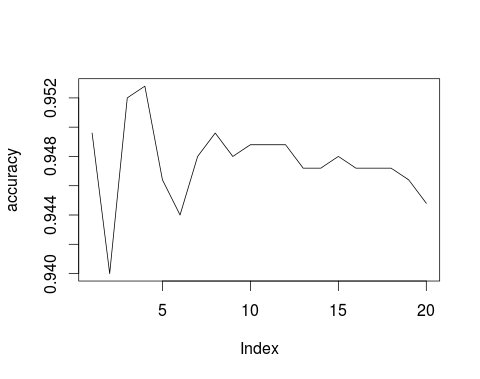
\includegraphics[width=0.5\textwidth]{img/KNN-Type(Not-Scaled).png}
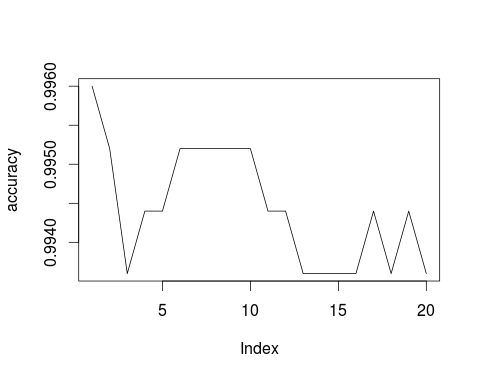
\includegraphics[width=0.5\textwidth]{img/KNN-Type(Scaled).png}
\caption{kNN - Type (With out and with the data scaled)}
\label{fig:KNN-TYPE}
\end{subfigure}

\begin{subfigure}[b]{\textwidth}
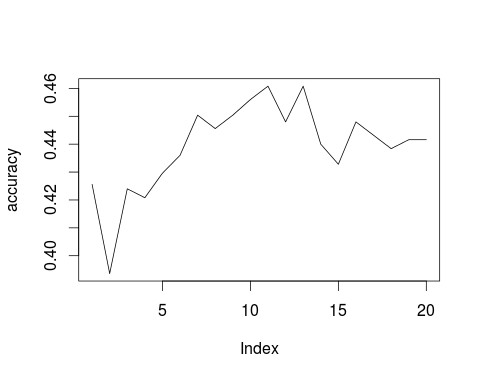
\includegraphics[width=0.5\textwidth]{img/KNN-Quality(Not-Scaled).png}
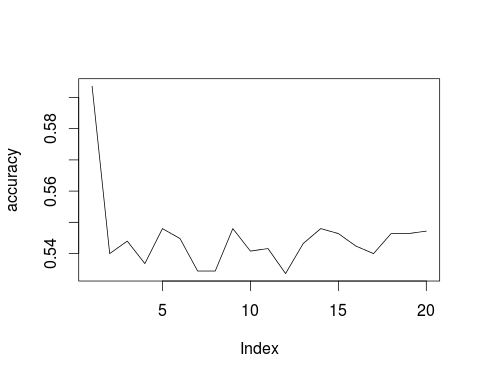
\includegraphics[width=0.5\textwidth]{img/KNN-Quality(Scaled).png}
\caption{kNN - Quality (With out and with the data scaled)}
\label{fig:KNN-Quality}
\end{subfigure}
\caption{Find k for the kNN}
\end{figure}



%----------------------------------------------------------------------------------------
\end{document}
